\documentclass{article}[12pt]
\usepackage{lipsum}
\usepackage{enumerate}
\usepackage{multicol,caption}
\usepackage{url}
\usepackage{graphicx}
\usepackage{wrapfig}
\usepackage[margin=2.5cm]{geometry}

\begin{document}
\title{Flight Quest: Flight Optimization, Paper 36}
\author{
	Group of 4
}
\date{}
\maketitle

\setlength{\columnsep}{1cm}
\begin{multicols}{2}

\section{Introduction}
In the modern day, airplanes are a frequently-used means of transportation. However, using it is fairly expensive to manage due to costs of fuel and delay. Due to many different factors, such as weather, restricted areas, and jet streams, it's very difficult to keep this cost of such transportation at an optimal level; airline companies are always looking for more ways to optimize their flights. What we aim to do here in Flight Quest 2 is to optimize to the best of our ability the costs of airplane flights using machine learning techniques on large sets of data. Flight Quest 2 is a competition on Kaggle hosted by General Electric. With thin margins, a small reduction in cost can cause large increases in profit. Reducing cost can also make flying easier for people and can also help the environment by reducing fuel burn. The goal in this competition is to create an agent that generates flight routes based on certain information given. The problem formulated is that the training data gives parameters such as flight routes and broadcasts from the airplane. In real life, we have all this information, up until a certain point in time. This is how the test data is structured. (perhaps we should move this) The goal is to create an agent that can advise pilots on optimal flight patterns. (let's add some sources about costs) (I think this can be combined with motivation)

\subsection{Motivation}
Our motivation for undertaking this task came from searching for something that would challenge us to apply what we learned in innovative ways, give us experience with working on a real-life machine learning problem, and give us an opportunity to have an impact on people's lives. The Flight Quest problem satiates these desires by starting us off at the beginning, giving us a goal, and then telling us to go about solving this problem however we deem necessary. It presents to us a problem that we have never encountered; a problem that requires learning to create optimization instead of classification. Therefore, our attempts at solving this problem are more centered around finding ways to extend and evolve the machine learning techniques that we've been using for other learning tasks rather than simply reuse them. This project requires more creativity as the literature on this problem is very limited. We also deal with the real-life issues of feature selection and generation. 
 
\section{Problem Definition and Methods}

\subsection{Task}
Our task finding least-cost paths for new flights to take from their current location to get to their location. We are given that the following things factor into calculating the cost of a flight:
	\begin{itemize}
		\item Fuel consumption
		\item Delay of flight arrival
		\item Crossing into restricted areas
		\item Changing the speed and altitude many times
	\end{itemize}
However, we are not given how much the factor in, and there are still more factors involved in the cost that aren't as clear-cut, such as turbulence and weather effects. The cost model is based on relative cost in dollars that tries to measure the direct and indirect costs of flights. Our goal is to construct a series of points (latitude and longitude) with airspeed and altitude labeled which correspond to the flight route.\\

In order to assist us in finding an optimal path, we have data from previous flights and other things such as airport and restricted area locations. However, the size of the data is very large (several gigabytes worth), meaning that we will have to be selective with what we use. Beyond this, there are no other guidelines to follow; we are free to approach the problem in any way necessary and use any resources that we need for our approach.\\
Each data release covers a certain time period. The data provides all information about flights: destination airport, arrival airport, scheduled and actual departure and arrival points, positions transmitted by the aircraft during flight, flight schedules and changes to said schedules. Also provided is weather conditions like runway conditions and sky conditions. \\
The test data is similar, but all are information is cut off after a certain time period. The collection of test flights is a list of flight IDs corresponding to flights in the test set along with current position, speed, altitude as well as certain delay costs and fuel costs. All test flights start above $18,000$ feet and are at least 75 miles away from the destination airport. They are all medium range aircraft. Flights are optimized independently so instructions for a flight are only used to simulate the cost of that one flight. \\
This problem is important because in this age big data can be seemingly used to optimize a processes so it is worth asking whether it can help airlines. This problem is interesting because we wonder whether an agent can indeed help pilots know which routes to follow. Structured output usually does not have set algorithms so we would need to do something somewhat unique. Another part of the task is selecting and possibly creating features. 

The competition is scored by submission onto a website. On their end, they run a simulator with weather data and ground conditions data which uses a physical model to simulate fuel burn using factors such as windspeed and distance traveled. Because of the nature of this, techniques such as cross validation tend to not work and overfitting is less of a concern because of the large hypothesis space and because the competition is scored with a random $57\%$ subset of the data used to calculate the leaderboard.
\subsection{Algorithms and Methods}

The basic goal in this case should be to create a series of points and classify them with altitude and speed for each aircraft. Our principal assumption is that the great-circle path should be the shortest, provided we avoid restricted zones which incur the same cost as the flight not reaching the destination. We see k-nearest neighbors as a very natural solution as well as ensemble methods due to their robustness.\\

We used Python 2.7 due to number of machine learning libraries and ease of scripting for splitting up data. We used SciKit Learn for most of our learning algorithms as well as GeoPy and Shapely for geometry related to the Earth. We also used Pandas to read in CSV files. We also used a chunk of code uploaded by a competition administrator on GitHub. We ran all our tests on Windows 7 x64.

\subsubsection{Restricted Zone Avoidance}

There were many reasons why our baseline did not produce the most optimal path, but the largest aspect we overlooked in our previous assumptions was the existence of restricted areas, which are locations on maps that passenger planes are not allowed to pass through i.e. passing through them would results in accumulating large amounts of cost. Therefore, we want to maintain the shortest path as we did with the baseline, but this time take into consideration the location of restricted areas.\\

We also tried out publicly released code by a competition administrator which attempting to avoid restricted zones by pushing the path away from the centroid of the restricted zone, but this was flawed.

Another way to avoid restricted zones is to follow our own path. In order to do this, we took the following approach: we generate using a uniform distribution many "waypoints" that lie between the current and detination location geographically. By producing a fine enough grid, we should have a very good approximation of the shortest path. Then, we utilize an A* search to find the shortest path from our current location to our destination location and avoid restricted zones by employing a distance function that sets the distance from any point to a point in a restricted zone to be very large.
\begingroup
  \captionof{figure}{Visualization of A* search.}
  \begin{center}
    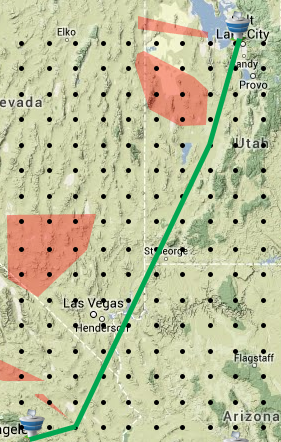
\includegraphics[width=1.5in]{astar.png}
	\end{center}
\endgroup

\subsubsection{Condition Optimization}
The distance that the path covers is only one factor for the cost; in order to have a complete flight plan, we must also include speeds and altitudes for each part of the flight plan. Both of these also affect the cost of our flight in many ways. For example, if the flight is on track to arrive on time, we don't want to unnecessarily expend fuel to get there faster. We also want our flight plans to be as consistent with these attributes as possible, since changing them multiple times incurs cost during the transitions. Keeping this in mind, we made several varying attempts in our approach. 

\subsubsection{Data Trimming and Feature Selection}

Before we began using any machine learning models, we had to determine how we would first handle the data. As stated before, the data provided to us is very large and contains some unimportant information, so training on a model using all of it is time-expensive. We first identified the features that were given by the test flights, which were substantially fewer than those given by the training flights and then took those into consideration. Afterwards, from these trimmed down features, we used those that would best match the method we used. 


\subsubsection{Whole Flight Classification}
For many flights, we made the assumption that for a certain distance of flight, there is an optimal speed and altitude to cruise at at which the airplane will follow for the majority of the route which excludes descent and ascent because the test flights file is always given for flights that have already taken off. For descent, we used a fixed distance and altitude.

\subsubsection{Ensemble Methods}
We used destination, distance until destination, and time until arrival as features here. Our thought was that optimal cruise altitude and speed would be based off the distance length of a flight because going to high altitudes would be less efficient for shorter flights because of the cost of fuel. Destination seems relevant because flights going to the same destination usually follow similar paths. Time until arrival is also a useful feature because it is correlated with speed and altitude since a late flight will want to get there faster.
\\

An advantage of ensemble methods is that they have low variance. In this way, outliers are unlikely which stops the flight taking odd paths. In addition, ensemble methods don't depend on a similarity measure and in general, we have found them to produce pretty consistent results without too much information about the features because most use averaging amongst decision trees.\\

We used random forests and gradient boosting. Random forests trains an ensemble of decision trees. The standard random forest uses a random subset for splitting criteria while the extremely random trees method uses a different random subset to evaluate the splitting criteria each time \cite{randomforest}. Gradient boosting trains an ensemble of random trees and uses a loss function to optimize the weights \cite{gradientboost}. 
\textbf{(mention which scikit learn things they are)}

\subsubsection{Point by Point Classification}

When we create our flight paths, we expect it to be segmentable into several parts based on the waypoints we expected the path to pass through. Therefore, another approach is rather than assume a single optimal speed and altitude for the flight, we can find the optimal speed and altitudes at each of these points for the flight. While this allows us to micromanage our flights more, we must also keep in mind that doing this will result in greater costs due to the fact that frequently changing these attributes incur cost during transitions.

\subsubsection{Ensemble Methods}

Similar to how we utilized ensemble methods before, we can use then here since the problem has effectively downscaled in size from a full path to points on a path. However, for this same reason, we cannot use the same features as before. Now, instead of using destination, distance until destination, and time until arrival, which were more oriented to give details of a full path, we will use the position of the waypoint, the direction that the flight is proceeding, and the distance from the destination. These features allow us to provide more details indicative of a point on a path while also giving an idea of how our overall path uses that point (i.e. identify it as a turning point, descent point, etc.).

\subsubsection{K Nearest Neighbors}

If we assume that our flight examples finished with an optimal path, then similar to how we approached the restricted zones problem, we can model our test flight by comparing it to a previous training flight. We simplified the problem to classify a series of points along the approximate shortest route that avoided restricted zones. From here, we classified the altitude based on latitude, longitude, and initial bearing (direction).\\

The intuition by creating bearing as a feature was that flights flying in different directions face different winds and thus have different efficiencies. We then used position, bearing, and altitude to determine the speed. We determined that speed mostly depended on altitude. To run this, we used SciKit-Learn's neighbors.nearestNeighborsRegression() model which uses Minkowski distance metric with $p=2$ and uses a ball-tree implementation to speed up search through a large space \cite{scikit}. We also split up the data by airport so that points would only be classified against flights going to the same airport to avoid issues with flights with low altitudes when passing by an airport.

\section{Evaluation}
\subsection{Methodology}
Since the goal is to create a path of least cost, our approach remains consistent in that we prioritize optimizing things that will have the biggest impact on the cost. However, since we don't know for sure all of the factors that go into calculating the cost nor how much each one is considered, we must also reorganize our plan based on assumptions made $\grave{a}$ $la$ a trial-and-error process.

\subsubsection{Baseline}

We used the simplest assumption for our baseline that since fuel was one of the considerations for calculating cost, so if we optimize the distance traveled (i.e. find the shortest-distance path), then we conserve fuel and as a result, lower our cost. However, since we are working with spherical coordinates instead of Euclidean coordinates, we must consider a different way of determining the shortest distance than what we are used to. For spherical coordinates, this distance is called the "great-circle" distance and is found by \cite{wiki}:\\

	\begin{enumerate}
		\item Finding the great circle on which the two points (current position and destination) lie.
		\item Separating the great circle into two arcs via the two points. 
		\item Taking the smaller of the two arcs.\\
	\end{enumerate}

Despite our assumptions, using this method to determine our answer incurred a cost that was significantly large. This is due to the fact that straight-line paths are susceptible to cross through restricted zones, as shown below.

\begingroup
  \captionof{figure}{Visualization of baseline approach.}
  \begin{center}
    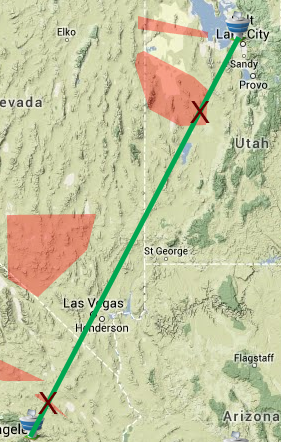
\includegraphics[width=1.5in]{baseline.png}
	\end{center}
\endgroup

\subsection{Results}
Due to the fact that our problem was one of optimization, the only way for us to analyze how "correct" our solution was was to utilize a cost calculator, which would take in a set of completed test flights and return a score based on the total cost incurred across all of the test flights. The full results can be found below, as well as how long the computations took for each method: \\

\begingroup
\noindent
\begin{tabular}{ | l | l | }
    \hline
    Method & Index \\ \hline
    Gradient boosted A* (single velocity) & 1\\ \hline
		RandomForest A*(single velocity) & 2 \\ \hline
		Unsmoothed Gradient Boost A* & 3 \\ \hline
		Unsmoothed kNN A* & 4 \\ \hline
		Smoothed weighted KNN A* & 5 \\ \hline
		Smoothed Forest of Random Trees A* & 6 \\ \hline
		Gradient boosted centroid avoider & 7\\ \hline
		Baseline & 8 \\ \hline
\end{tabular}
\begin{center}
    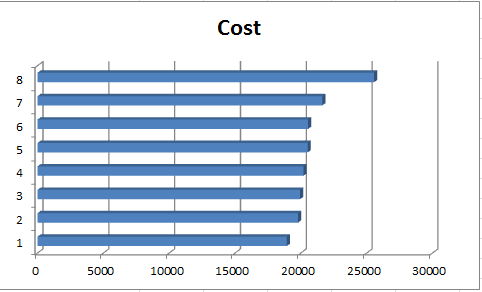
\includegraphics[width=3in]{results.png}
		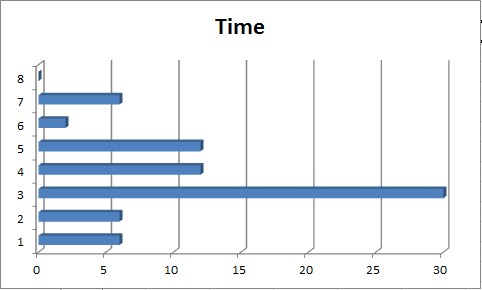
\includegraphics[width=3in]{time.png}
	\end{center}
\captionof{figure}{Our cost values for the methods we tried.}
\endgroup

\subsection{Discussion}
In general, the algorithms seem to produce reasonable paths. Some of the paths seem to be sensitive to outliers, though, resulting in suboptimal paths. Many of the methods we used produced comparable costs, so it's not unreasonable to think that, with better tuning, that some of them could turn out to be a reliable solution. However, as we can see from the time it takes to compute each method, undergoing the process for some methods will be drastically more time-expensive than doing the same for others. It's also worth noting that the two best methods we've tried so far: gradient boosted A* and random forest A*, both have a relatively short computation time of 6 hours, meaning that doing computations in a greater amount of detail does not necessarily give us a better solution.  

\section{Related Work}
We were not able to find any academic literature on this. We were able to peruse the forums for this competition and milestone version of it. Top-ranked submissions for the milestone used the data to train for optimal cruise speed and altitude. They also trained for optimal descent. Some used a cost-based model. The milestone competition winner used a cost based model which considered only the features that could reduce fuel burn. 

\section{Future Work}
While we have done work and seen improvements, a lot can be done. It is likely that optimal routes may not just the shortest geographic distance due to winds. But the winds of the future cannot be known ahead of time. Being able to forecast wind and relating a cost function to wind over the entire geographic map may allow an improvement in path. One way may to be use KNN to see what direction a plane at the current point will head. This is a bit problematic though as bearing changes along a great-circle path from one point to another. Initial bearing may be used or perhaps the classification should be what waypoint should the plane head to next. It may also help to consider other methods in classification of speed and altitude. Currently, fuel cost and delay cost is not present in our model. These features, if added, could definitely yield improvements but the question of how to implement them is varied since there is not a direct cost to fuel cost relation and the cost of delays and fuel is not included in the training data. The optimal way would likely be to incorporate this into our model as parameters that can be tweaked with weights in a higher level learning problem to determine the optimal weights. \\

Another issue is the presence of outliers in our data classification. Inspecting our paths, most paths seem very reasonable but sometimes outliers are present in the data where a plane goes from 36000 feet altitude to 8000 feet to 36000 feet in two steps. Detecting changes like this aren't quite that simple. It may be possible to train these using some type of Markov model where the probability of different percentage based or absolute altitude changes are calculated and we tweak the confidence that this is a mistake to smooth the data. Then, the middle point could be the arithmetic or geometric mean of the two points' altitudes.

\section{Conclusion}
In the end, we were able to get some improvement compared to the baseline mode, but we are still far off from the leaders of the competition. We have illustrated that machine learning can be used to some extent to plan flight routes, but perhaps some optimization techniques are needed as well. Feature selection is difficult and large datasets are hard to work with because of not only dealing with the data, but because of runtime issues, our choices for learning algorithms are limited. We tried Support Vector Regression, but the runtime was completely unreasonable even on a small subset. Our results show that machine learning can be applicable to optimization.


\begin{thebibliography}{1}

\bibitem{kaggle} "Description-Flight Quest 2: Flight Optimization | GE Quest". \url{http://www.gequest.com/c/flight2-main}.
\bibitem{forum} "Flight Quest 2: Flight Optimization Forum | GE Quest". \url{https://www.gequest.com/c/flight2-milestone/forums}.
\bibitem{wiki} "Great-circle Distance". \url{http://en.wikipedia.org/wiki/Great-circle_distance}.
\bibitem{scikit} "scikit-learn: machine learning in Python". \url{http://scikit-learn.org/stable/}.
\bibitem{geopy} "geopy-A Geocoding Toolbox for Python". \url{https://code.google.com/p/geopy/}.
\bibitem{pandas} "Python Data Analysis Library". \url{http://pandas.pydata.org/}.
\bibitem{shapely} "Shapely 1.2.18: Python Package Index". \url{https://pypi.python.org/pypi/Shapely}.
\bibitem{randomforest} "Random Forest". \url{http://en.wikipedia.org/wiki/Random_forest}.
\bibitem{gradientboost} "Gradient Boosting". \url{http://en.wikipedia.org/wiki/Gradient_boosting}.
\bibitem{hamner} "GE Flight Quest 2 Basic Agents". \url{https://github.com/benhamner/GEFlight2BasicAgents}.
\end{thebibliography}
\end{multicols}
\end{document}